\documentclass[tikz,10pt]{standalone}
\usepackage{tkz-euclide}

\definecolor{ccred}{cmyk}{0, 0.87, 0.8, 0.21}
\definecolor{ccgreen}{RGB}{147,187,42}
\definecolor{ccgrey}{RGB}{158,155,155}
\definecolor{violet1}{RGB}{153,0,153}

\begin{document}
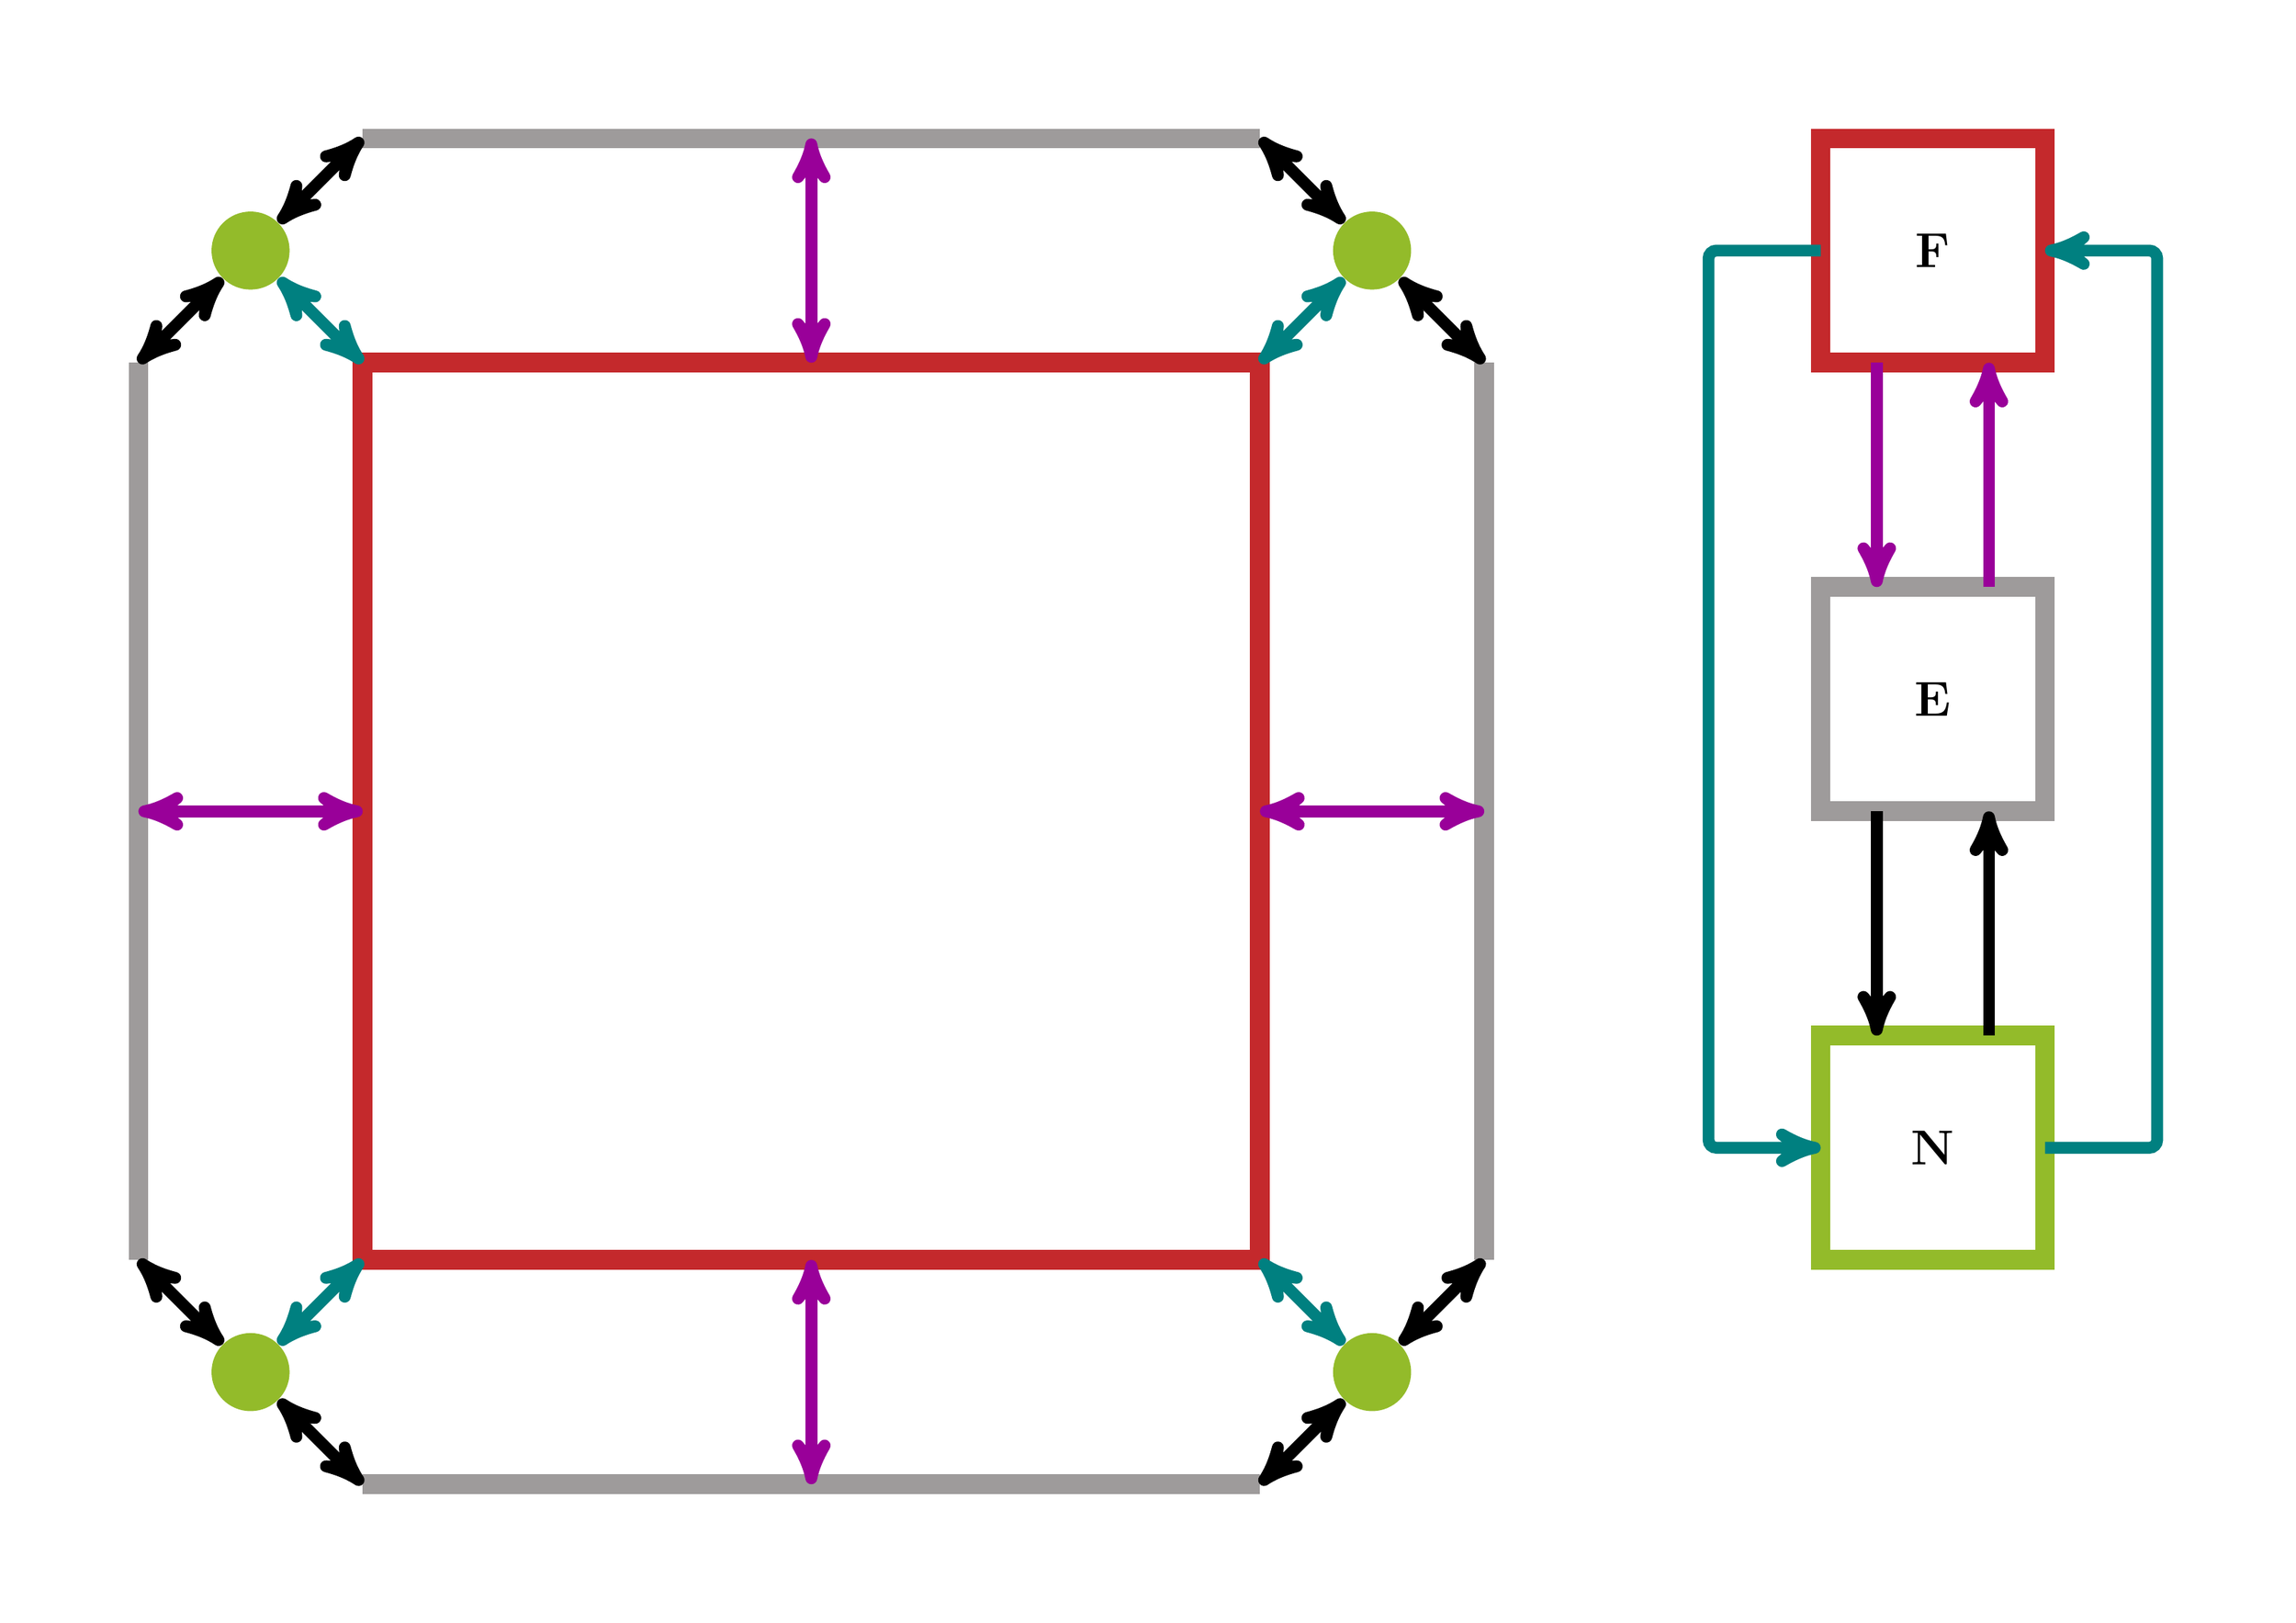
\begin{tikzpicture}[scale=2]

   % Style des flèches
  \tikzstyle{fleche} = [->, >=stealth', thick, rounded corners=4pt]
  \tikzstyle{doublefleche} = [<->, >=stealth', thick, rounded corners=4pt, line width=2]

  % Boîte englobante du schéma
  \draw (-7,-7) node (0) {} ;
  \draw (13,7) node (1) {} ;

  % Face
  \draw[line width=10, ccred] (-4,-4) -- (4,-4) -- (4,4) -- (-4,4) -- cycle ;
  
  % Noeuds
  \draw (-5,-5) node[circle, fill=ccgreen, inner sep=14pt] (n1) {} ;
  \draw (-5,5) node[circle, fill=ccgreen, inner sep=14pt] (n2) {} ;
  \draw (5,5) node[circle, fill=ccgreen, inner sep=14pt] (n3) {} ;
  \draw (5,-5) node[circle, fill=ccgreen, inner sep=14pt] (n4) {} ;

  % Arêtes
  \draw[line width=10, ccgrey] (-6,-4) -- (-6,4);
  \draw[line width=10, ccgrey] (6,-4) -- (6,4);
  \draw[line width=10, ccgrey] (-4,6) -- (4,6);
  \draw[line width=10, ccgrey] (-4,-6) -- (4,-6);


  % Connectivités F <-> N
  \draw[doublefleche, green!50!blue, line width=6] (n1) -- (-4,-4) ;
  \draw[doublefleche, green!50!blue, line width=6] (n2) -- (-4,4) ;
  \draw[doublefleche, green!50!blue, line width=6] (n3) -- (4,4) ;
  \draw[doublefleche, green!50!blue, line width=6] (n4) -- (4,-4) ;

  % Connectivités F <-> E
  \draw[doublefleche, violet1, line width=6] (0,4) -- (0,6) ;
  \draw[doublefleche, violet1, line width=6] (0,-4) -- (0,-6) ;
  \draw[doublefleche, violet1, line width=6] (4,0) -- (6,0) ;
  \draw[doublefleche, violet1, line width=6] (-4,0) -- (-6,0) ;

  % Connectivités E <-> N
  \draw[doublefleche, line width=6] (n1) -- (-6,-4) ;
  \draw[doublefleche, line width=6] (n1) -- (-4,-6) ;
  \draw[doublefleche, line width=6] (n2) -- (-6,4) ;
  \draw[doublefleche, line width=6] (n2) -- (-4,6) ;
  \draw[doublefleche, line width=6] (n3) -- (6,4) ;
  \draw[doublefleche, line width=6] (n3) -- (4,6) ;
  \draw[doublefleche, line width=6] (n4) -- (6,-4) ;
  \draw[doublefleche, line width=6] (n4) -- (4,-6) ;
  
  % Liste des boxes
  \draw[line width=10, ccred] (9,4) -- (9,6) -- (11,6) -- (11,4) -- cycle ;
  \draw[line width=10, ccgrey] (9,0) -- (9,2) -- (11,2) -- (11,0) -- cycle ;
  \draw[line width=10, ccgreen] (9,-4) -- (9,-2) -- (11,-2) -- (11,-4) -- cycle ;

  \draw (10,5) node (face) {\Huge \textbf{F}};
  \draw (10,1) node (arete) {\Huge \textbf{E}};
  \draw (10,-3) node (node) {\Huge \textbf{N}};

  % N <-> F
  \draw[fleche, line width=6, green!50!blue] (9,5) -- (8,5) -- (8,-3) -- (9,-3) ;
  \draw[fleche, line width=6, green!50!blue] (11,-3) -- (12,-3) -- (12,5) -- (11,5) ;
  % F <-> E
  \draw[fleche, line width=6, violet1] (9.5,4) -- (9.5,2) ;
  \draw[fleche, line width=6, violet1] (10.5,2) -- (10.5,4) ;
  % E <-> N
  \draw[fleche, line width=6] (9.5,0) -- (9.5,-2) ;
  \draw[fleche, line width=6] (10.5,-2) -- (10.5,0) ;

\end{tikzpicture}
\end{document}